\FloatBarrier
\subsubsection{Przykład}
\begin{figure}[h]
	\centering
	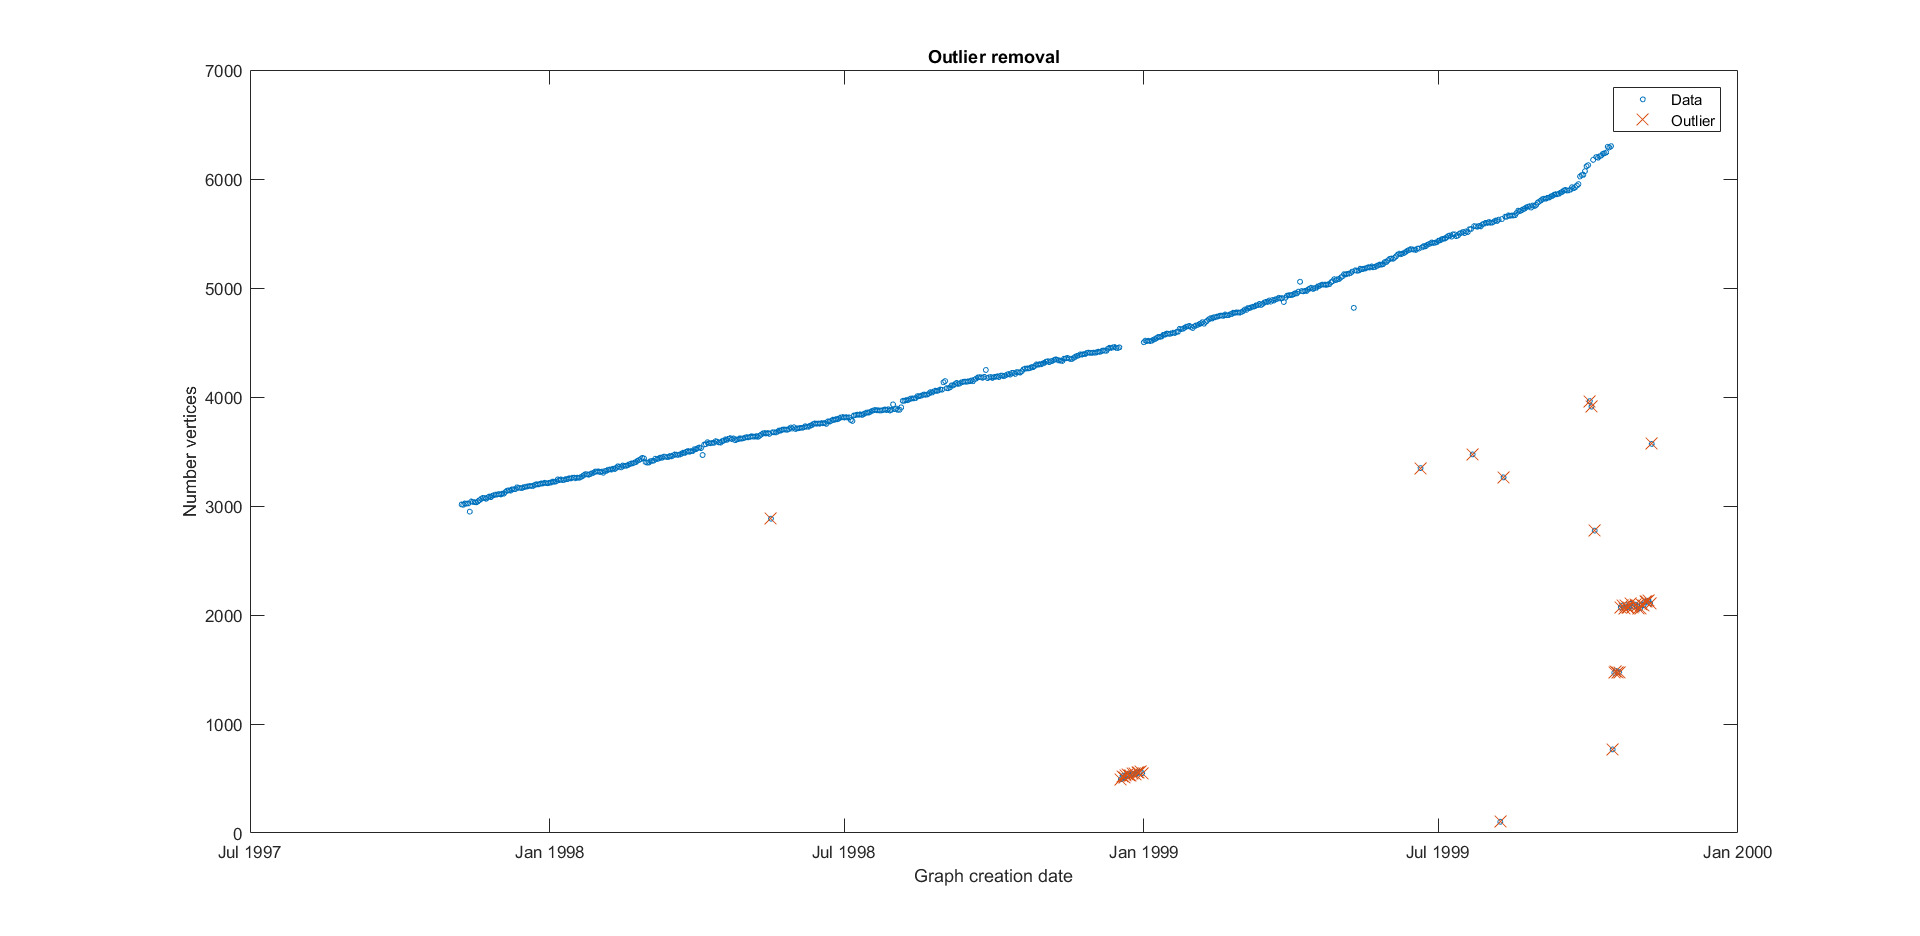
\includegraphics[width=\textwidth]{Outliers}
	\caption{Działanie Betweenness Centrality  na przykładowym grafie}
\end{figure}
\FloatBarrier
\subsubsection{Przykład}
\begin{figure}[h]
	\centering
	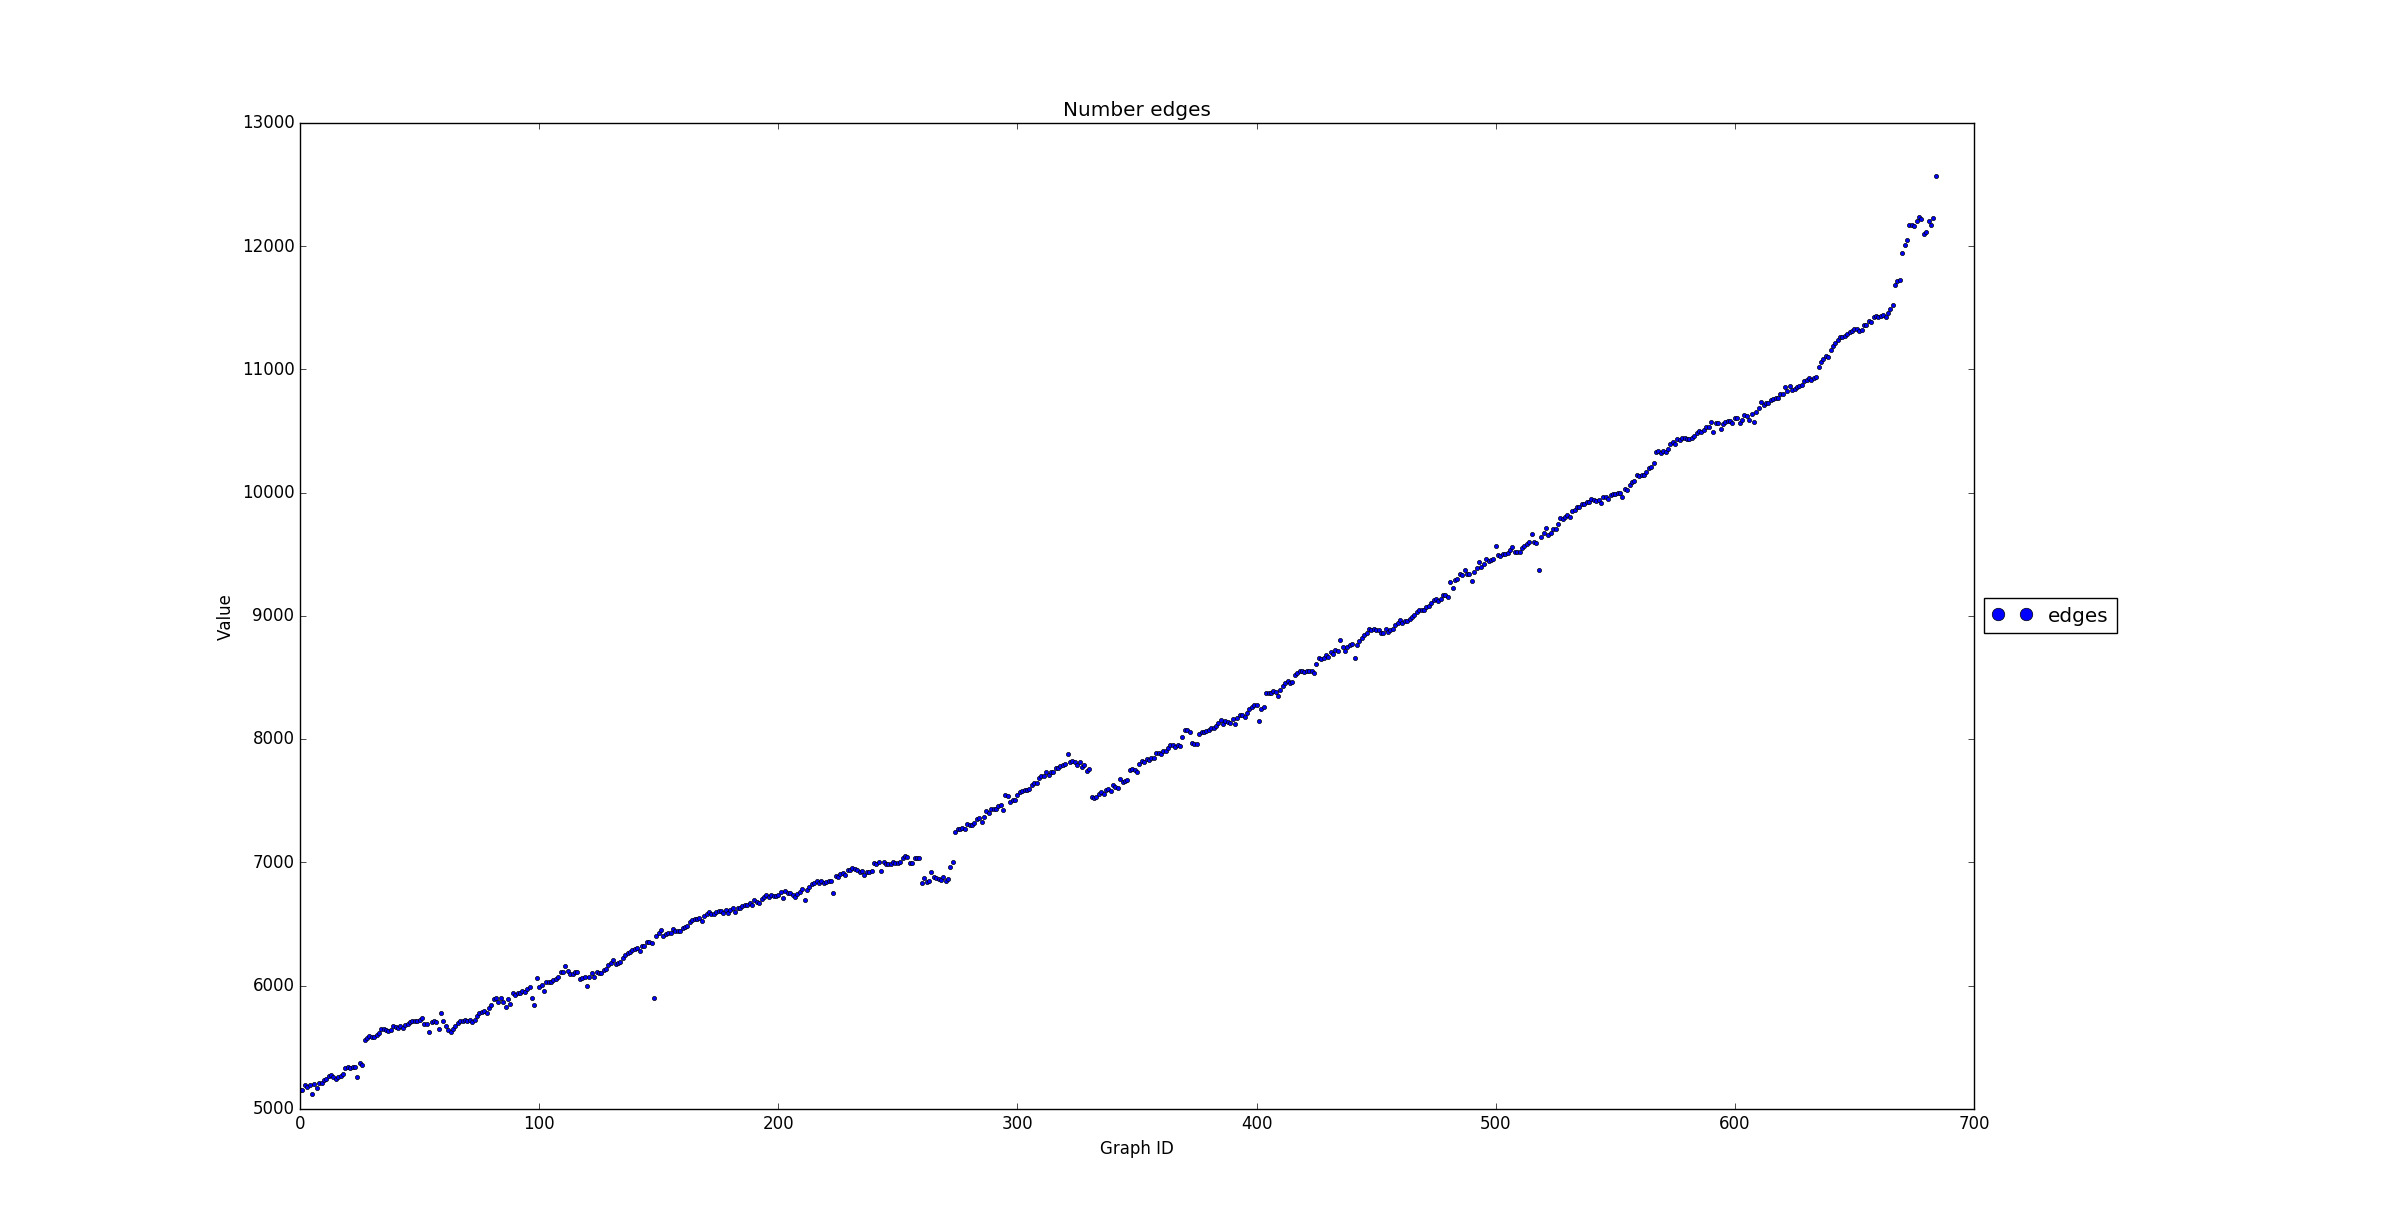
\includegraphics[width=\textwidth]{number_edges}
	\caption{Działanie Betweenness Centrality  na przykładowym grafie}
\end{figure}
\FloatBarrier
\FloatBarrier
\subsubsection{Przykład}
\begin{figure}[h]
	\centering
	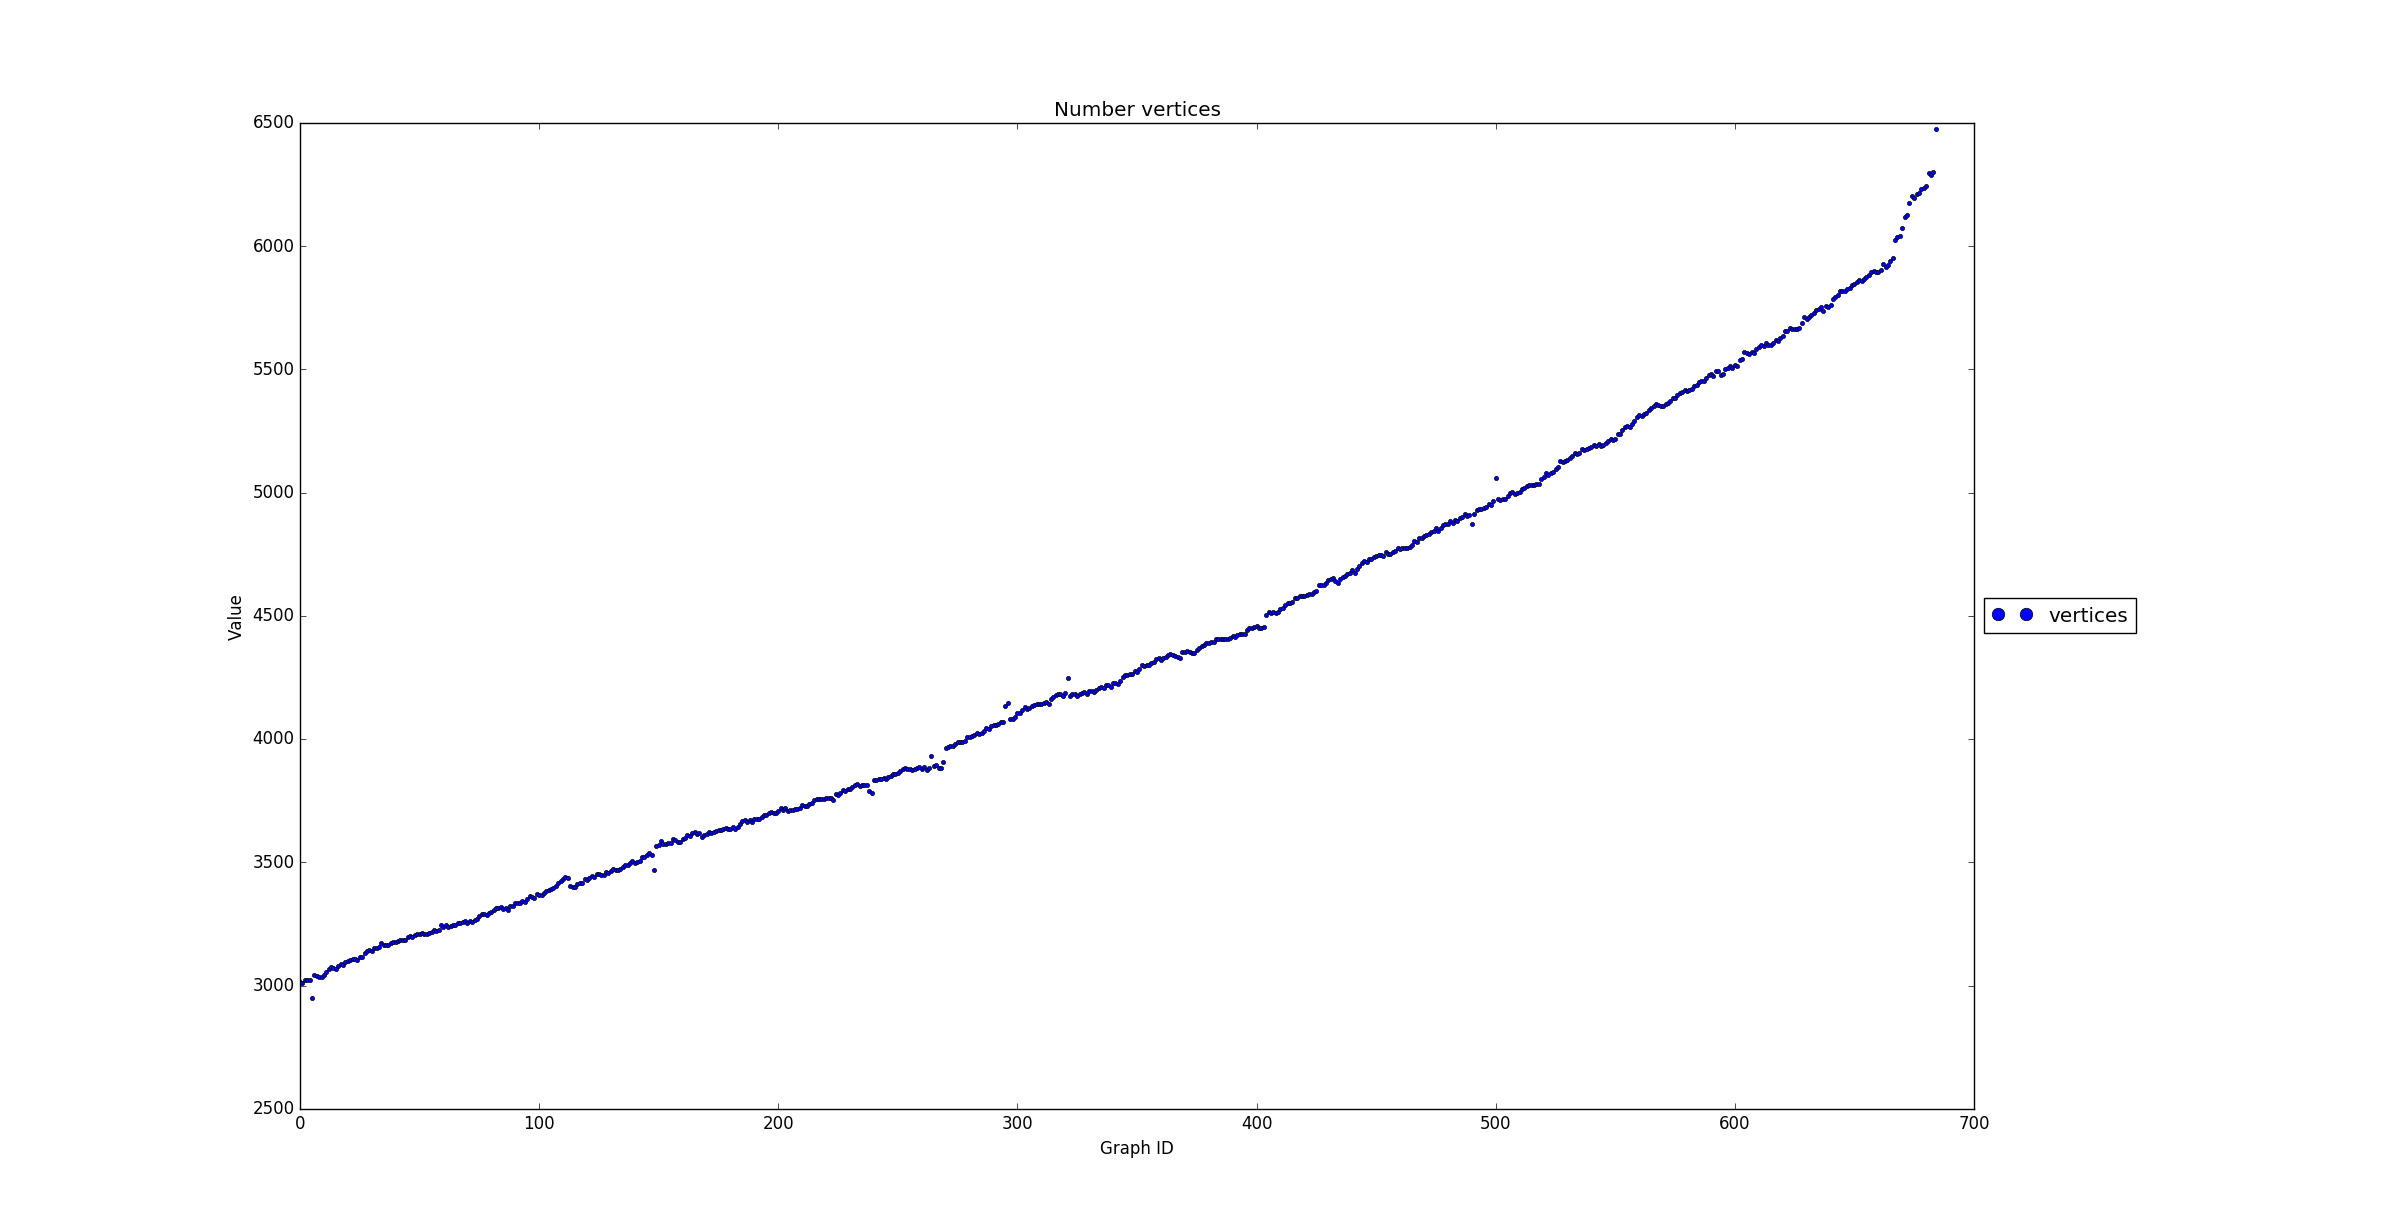
\includegraphics[width=\textwidth]{number_vertices}
	\caption{Działanie Betweenness Centrality  na przykładowym grafie}
\end{figure}
\FloatBarrier
\FloatBarrier
\subsubsection{Przykład}
\begin{figure}[h]
	\centering
	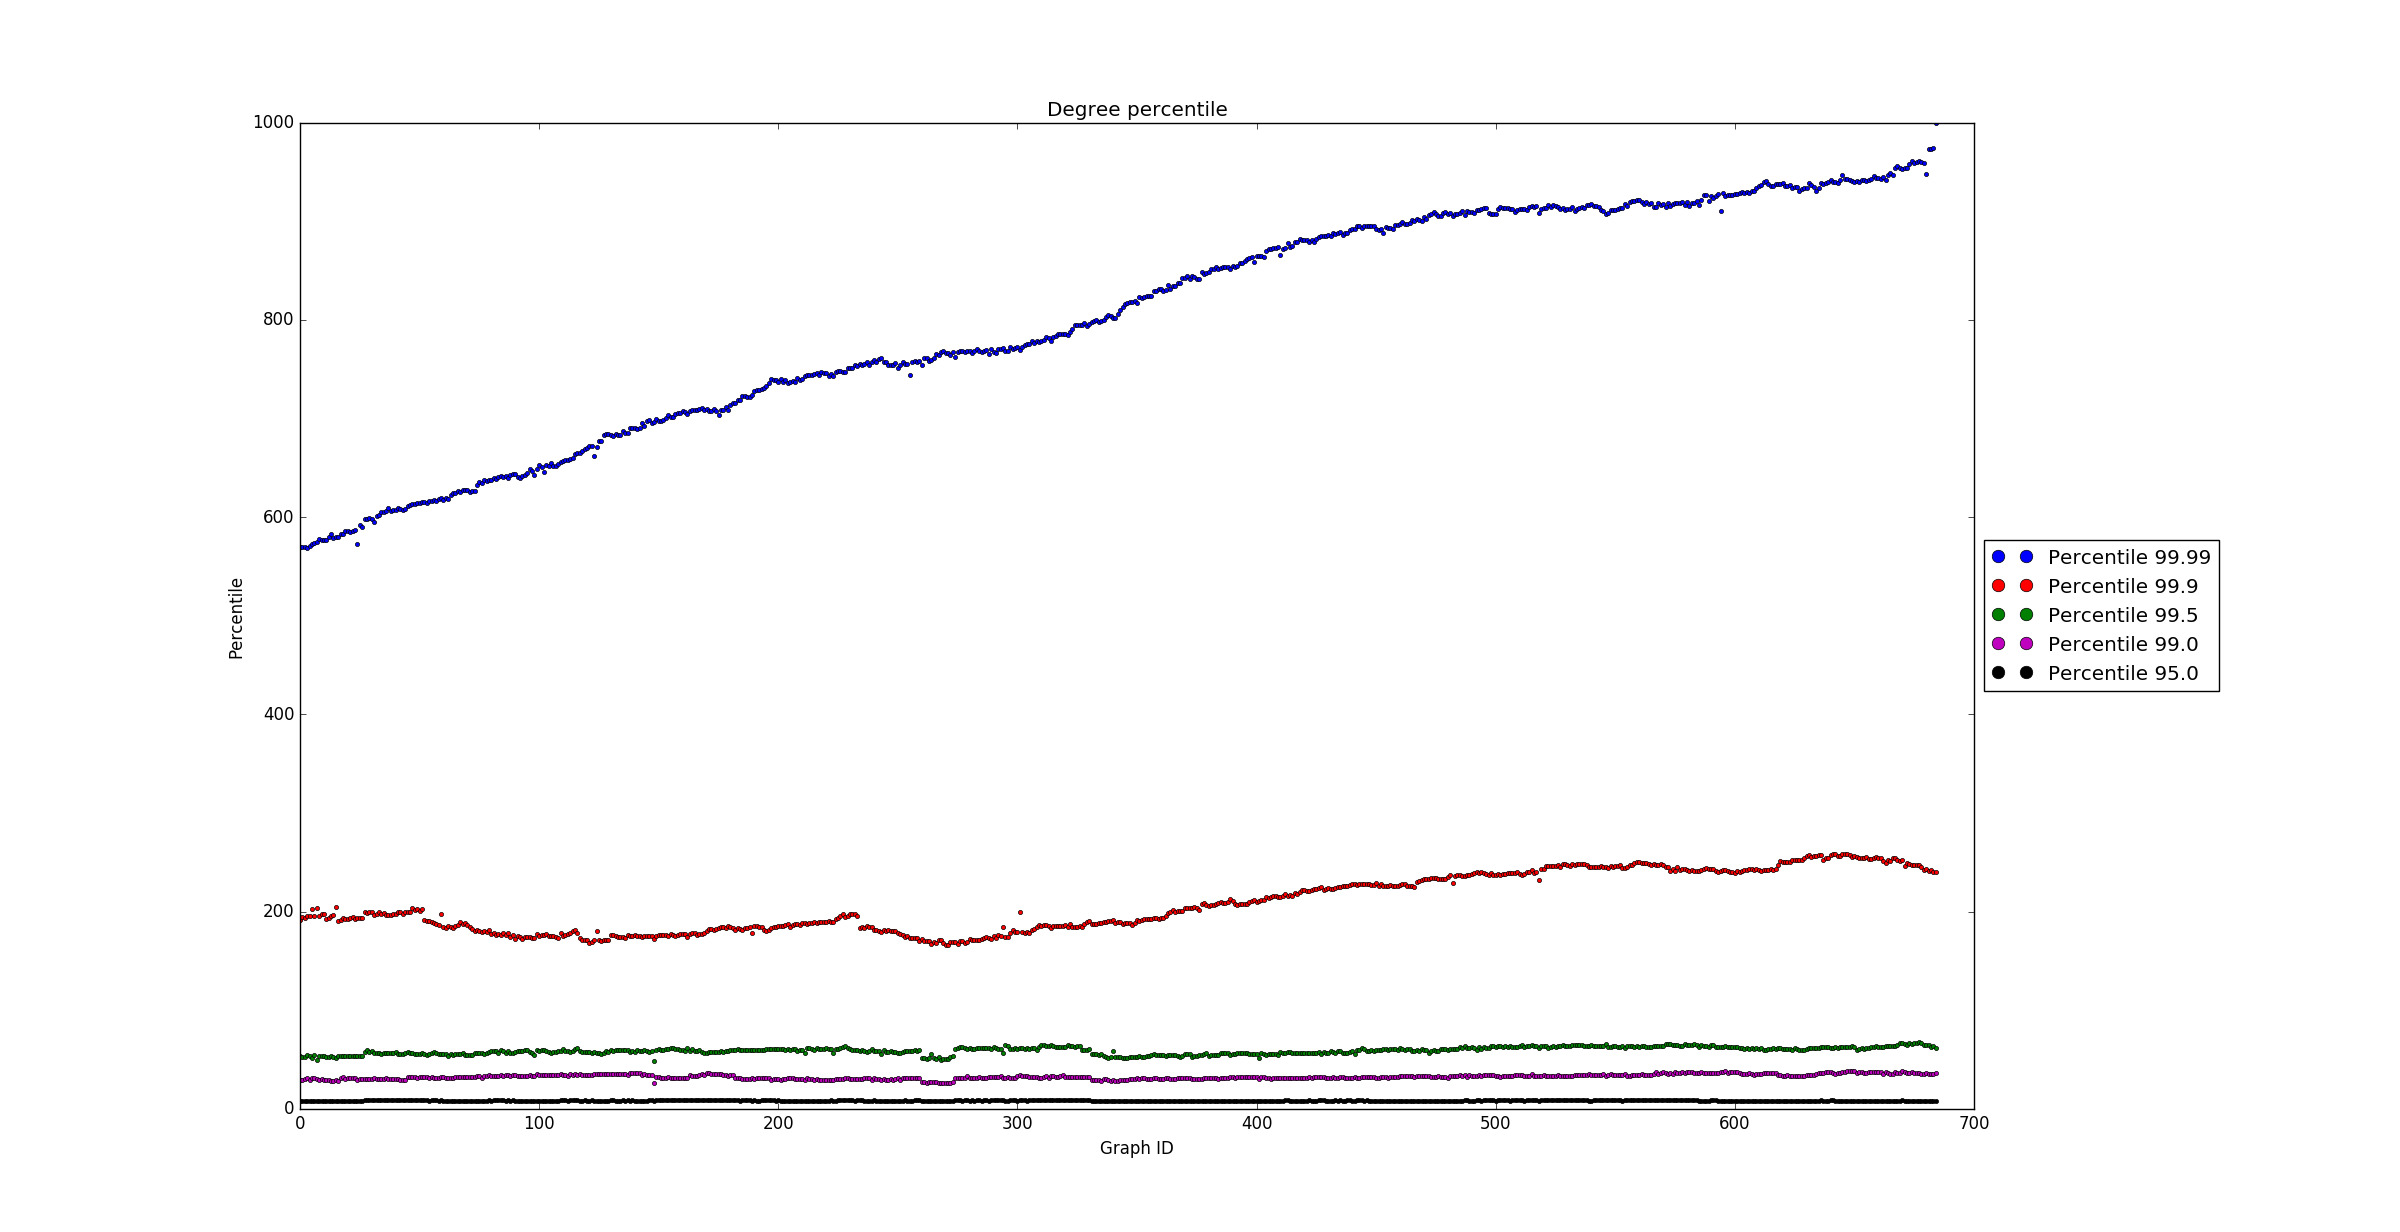
\includegraphics[width=\textwidth]{degree_percentiles}
	\caption{Działanie Betweenness Centrality  na przykładowym grafie}
\end{figure}
\FloatBarrier\FloatBarrier
\subsubsection{Przykład}
\begin{figure}[h]
	\centering
	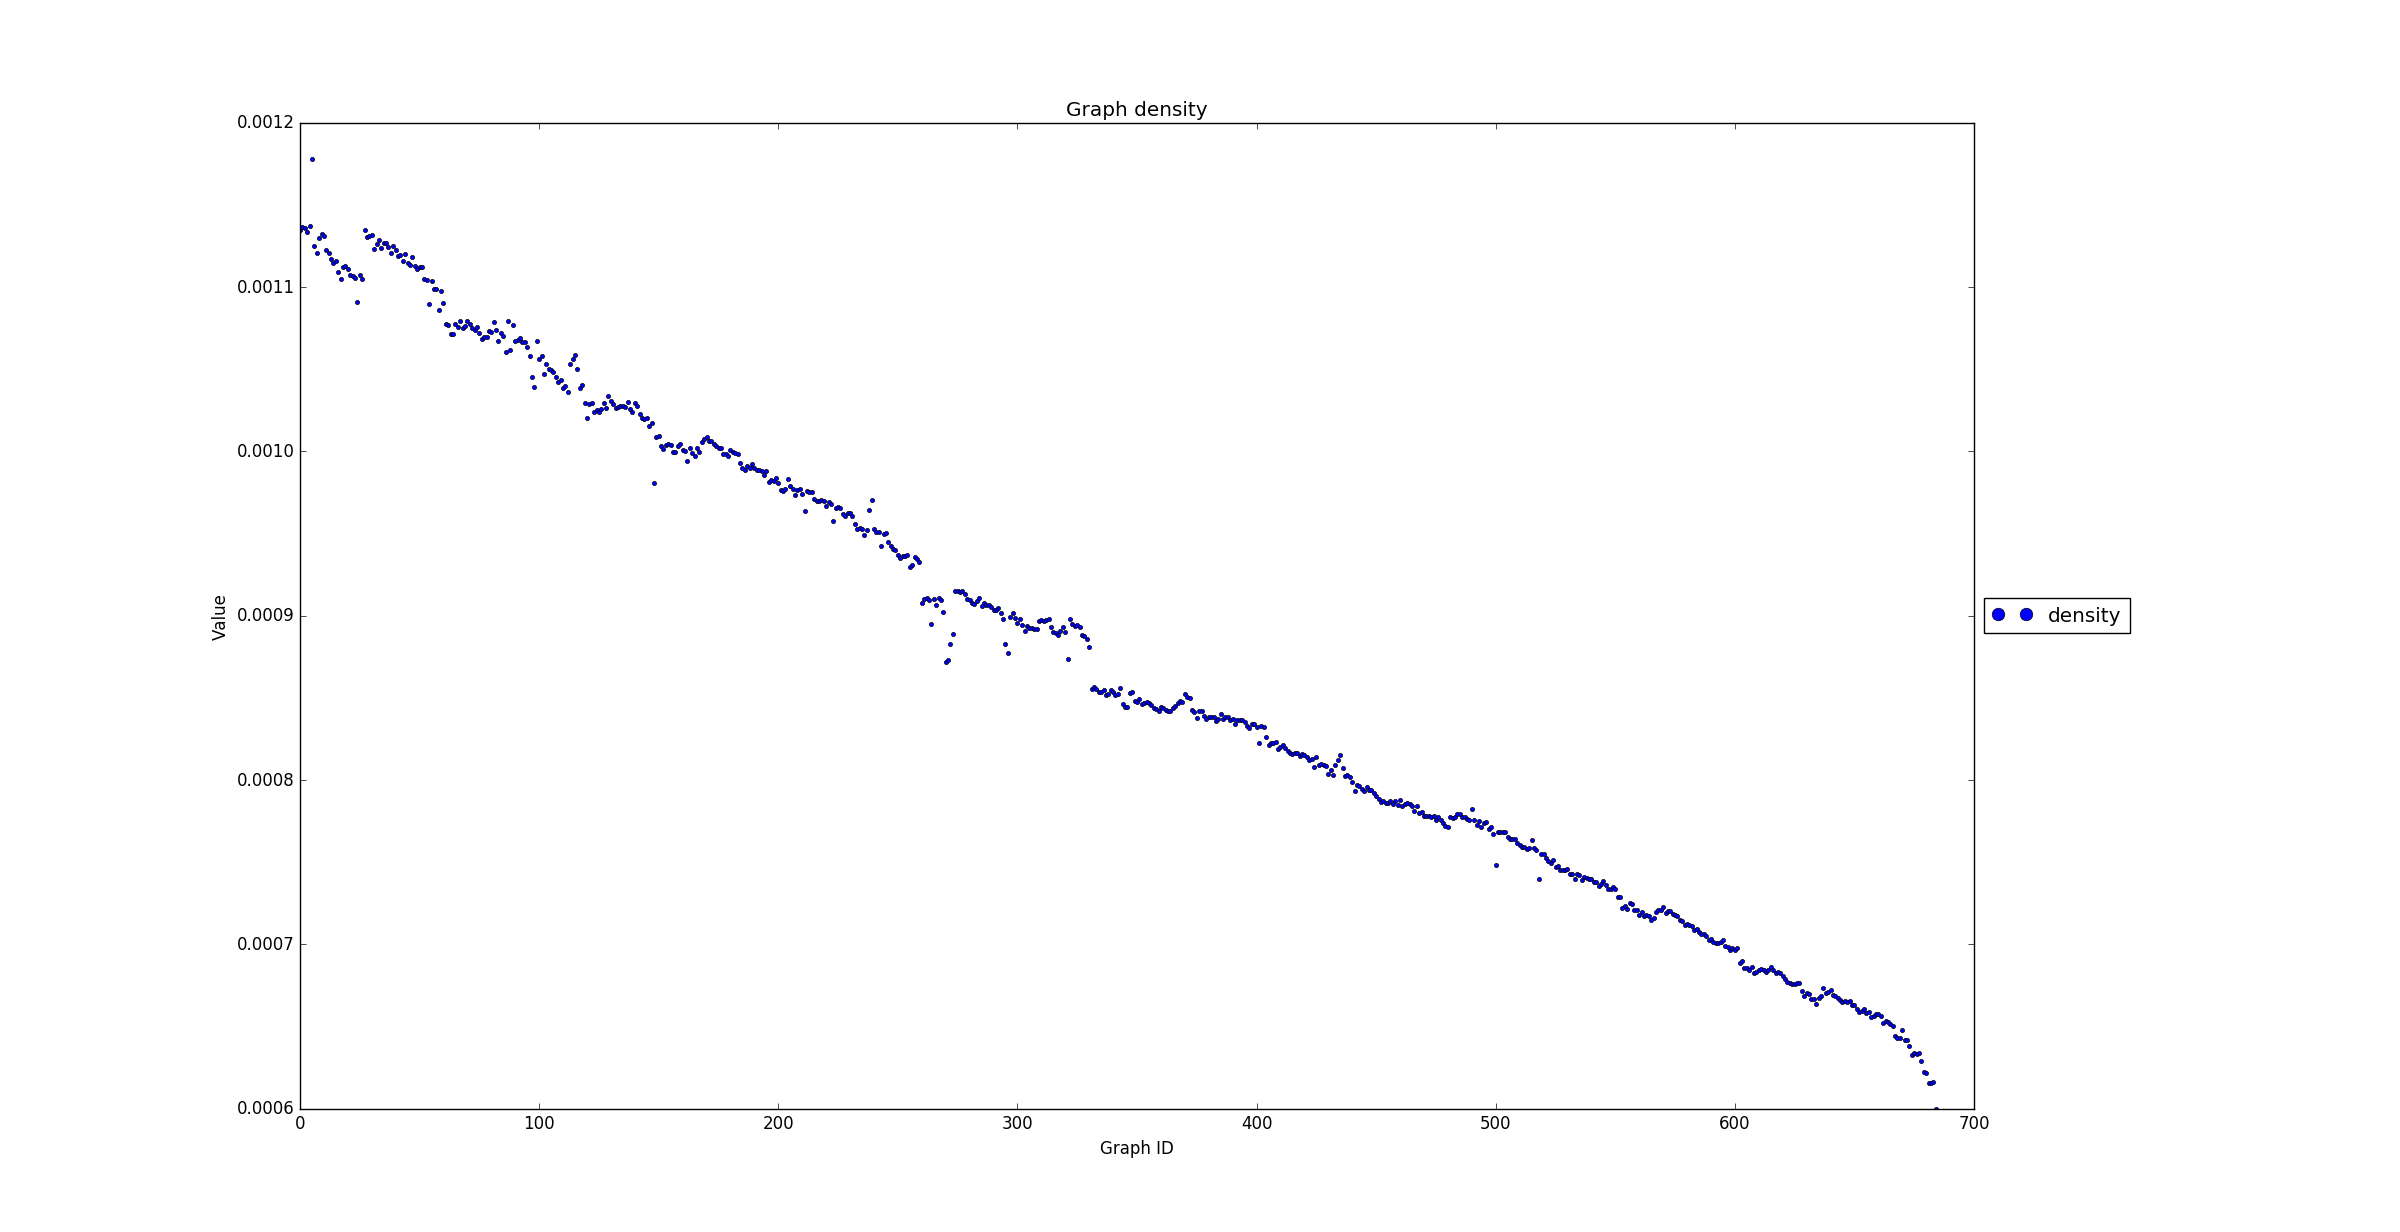
\includegraphics[width=\textwidth]{graph_density}
	\caption{Działanie Betweenness Centrality  na przykładowym grafie}
\end{figure}
\FloatBarrier\FloatBarrier